\subsection{Glyph: \glyph{Simple chemical activity}}
\label{sec:af:simpleChemicalActivity}

A simple chemical activity in SBGN Activity Flow is defined as the activity from a chemical compound that is not formed by the covalent linking of pseudo-identical residue, as opposite of a macromolecule activity (\sect{af:macromolecule}). Examples of simple chemicals are an atom, a monoatomic ion, a salt, a radical, a solid metal, a crystal, etc.

\begin{glyphDescription}

\glyphSboTerm SBO:

\glyphContainer A \glyph{simple chemical activity} is represented by a “stadium” shape, that is two semicircles of the same
radius joined by parallel line segments, as shown in \fig{af:simpleChemicalActivity}. If desired the parallel line segments can have zero length, and the shape is then identical to a circle. To avoid confusion with the unspecified entity (\ref{sec:unspecifiedEntity}), this form of the glyph must remain a circle and cannot be deformed into an ellipse.

\glyphLabel The identification of the \glyph{simple chemical activity} is carried by an unbordered box containing a string of characters.  The characters may be distributed on several lines to improve readability, although this is not mandatory.  The label box has to be attached to the center of the circular container.  The label is permitted to spill outside the container.

\glyphAux A \glyph{simple chemical activity} may be decorated with one or more \glyph{units of information} (\sect{af:unitInfo}). 

\end{glyphDescription}

\begin{figure}[H]
  \centering
  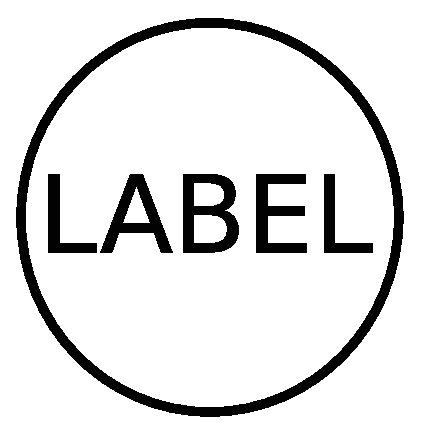
\includegraphics[scale = 0.3]{images/simpleChemical}
  \caption{The \AF glyph for \glyph{simple chemical activity}.}
  \label{fig:af:simpleChemicalActivity}
\end{figure}
